\documentclass{standalone}
\usepackage{tikz}
\usetikzlibrary{arrows.meta, positioning, shapes.geometric, calc,patterns}

\begin{document}
	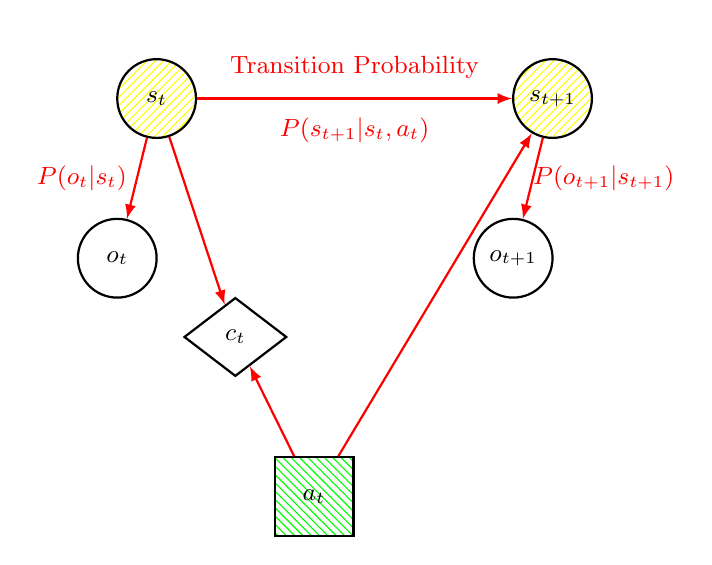
\begin{tikzpicture}[
		node distance=2cm and 1.5cm,
		every node/.style={minimum size=10mm, font=\small},
		cost/.style={draw,diamond, aspect=2, fill=white},
		state/.style={draw,circle,pattern=north east lines, pattern color=yellow},
		obs/.style={draw,circle, fill=white},
		action/.style={draw,rectangle, ,pattern=north west lines, pattern color=green},
		->, >=Stealth, thick, black
		]
		% Simple Influence diagram
		\node[cost] at (0,0) (cost) {$c_t$};
		\node[state, above = of cost,xshift = -10mm] (state) {$s_t$};
		\node[obs,below = of state, xshift = -5mm,yshift = 10mm] (obs) {$o_t$};
		\node[action,below = of obs,xshift = 25mm] (action) {$a_t$};
		
		\node[state,right = of state, xshift = 25mm] (statenext) {$s_{t+1}$};
		\node[obs,below = of statenext, xshift = -5mm,yshift = 10mm] (obsnext) {$o_{t+1}$};
		%		\node[obs] at (0,0) (obs) {$o$};	
		%		\node[action, right = of obs] (action){$a$};
		%		\node[state, below = of obs] (state){$s$};
		%		\node[cost, right = of state] (cost) {$c$};
		%		
		% Draw the causality arrows
		%\draw[-latex,red] (obs)--(action);
		\draw[-latex,red] (action) -- (cost);
		\draw[-latex,red] (state) -- (cost);
		\draw[-latex,red] (state) -- node[xshift = -7mm]{$P(o_t|s_t)$}(obs);
		\draw[-latex,red] (state) --node[xshift = 0mm,yshift = 4mm]{Transition Probability }node[xshift = 0mm,yshift = -4mm]{$ P(s_{t+1}|s_t,a_t)$} (statenext) ;
		\draw[-latex,red] (statenext) --node[xshift = 9mm]{$P(o_{t+1}|s_{t+1})$}(obsnext);
		\draw[-latex,red] (action) -- (statenext);
		% denote
		%		\node[draw = white,right = of cost,align=center,xshift= -22mm,yshift = 14mm]  {Cost \\negative Reward};
		%		
		%		\node[draw = white, left = of state,align = center,xshift= 10mm] {State};
		%		
		%		\node[draw = white, left = of obs,align = center,xshift= 10mm]  {Output from \\ SHM result};
		%		
		%		\node[draw = white, below = of action, align=center,xshift= -5mm,yshift= 20mm] {Action or Decision };
		
		
	\end{tikzpicture}
\end{document}
